% Ratio of the number of k-term progressions of primes to the Green-Tao-Ziegler prediction (generated by a script).
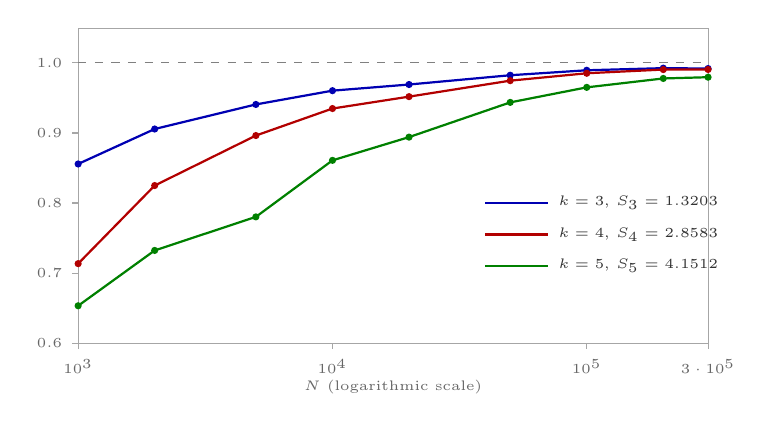
\begin{tikzpicture}[x=1cm,y=1cm]
\draw[black!35] (0,0) rectangle (8.00,4.00);
\draw[black!35] (0,0.00)--(-0.08,0.00) node[left,font=\tiny,black!60]{$0.6$};
\draw[black!35] (0,0.89)--(-0.08,0.89) node[left,font=\tiny,black!60]{$0.7$};
\draw[black!35] (0,1.78)--(-0.08,1.78) node[left,font=\tiny,black!60]{$0.8$};
\draw[black!35] (0,2.67)--(-0.08,2.67) node[left,font=\tiny,black!60]{$0.9$};
\draw[black!35] (0,3.56)--(-0.08,3.56) node[left,font=\tiny,black!60]{$1.0$};
\draw[black!35] (0.00,0)--(0.00,-0.08) node[below,font=\tiny,black!60]{$10^3$};
\draw[black!35] (3.23,0)--(3.23,-0.08) node[below,font=\tiny,black!60]{$10^4$};
\draw[black!35] (6.46,0)--(6.46,-0.08) node[below,font=\tiny,black!60]{$10^5$};
\draw[black!35] (8.00,0)--(8.00,-0.08) node[below,font=\tiny,black!60]{$3\cdot10^5$};
\node[below,font=\tiny,black!60] at (4.00,-0.35) {$N$ (logarithmic scale)};
\draw[black!50,dashed] (0,3.56)--(8.00,3.56);
\draw[blue!70!black,thick] (0.000,2.276) -- (0.972,2.720) -- (2.257,3.032) -- (3.230,3.207) -- (4.202,3.285) -- (5.487,3.403) -- (6.459,3.466) -- (7.431,3.493) -- (8.000,3.488);
\fill[blue!70!black] (0.000,2.276) circle (1.3pt);
\fill[blue!70!black] (0.972,2.720) circle (1.3pt);
\fill[blue!70!black] (2.257,3.032) circle (1.3pt);
\fill[blue!70!black] (3.230,3.207) circle (1.3pt);
\fill[blue!70!black] (4.202,3.285) circle (1.3pt);
\fill[blue!70!black] (5.487,3.403) circle (1.3pt);
\fill[blue!70!black] (6.459,3.466) circle (1.3pt);
\fill[blue!70!black] (7.431,3.493) circle (1.3pt);
\fill[blue!70!black] (8.000,3.488) circle (1.3pt);
\draw[red!70!black,thick] (0.000,1.010) -- (0.972,2.002) -- (2.257,2.637) -- (3.230,2.980) -- (4.202,3.131) -- (5.487,3.334) -- (6.459,3.428) -- (7.431,3.475) -- (8.000,3.476);
\fill[red!70!black] (0.000,1.010) circle (1.3pt);
\fill[red!70!black] (0.972,2.002) circle (1.3pt);
\fill[red!70!black] (2.257,2.637) circle (1.3pt);
\fill[red!70!black] (3.230,2.980) circle (1.3pt);
\fill[red!70!black] (4.202,3.131) circle (1.3pt);
\fill[red!70!black] (5.487,3.334) circle (1.3pt);
\fill[red!70!black] (6.459,3.428) circle (1.3pt);
\fill[red!70!black] (7.431,3.475) circle (1.3pt);
\fill[red!70!black] (8.000,3.476) circle (1.3pt);
\draw[green!50!black,thick] (0.000,0.475) -- (0.972,1.178) -- (2.257,1.604) -- (3.230,2.322) -- (4.202,2.617) -- (5.487,3.058) -- (6.459,3.249) -- (7.431,3.362) -- (8.000,3.378);
\fill[green!50!black] (0.000,0.475) circle (1.3pt);
\fill[green!50!black] (0.972,1.178) circle (1.3pt);
\fill[green!50!black] (2.257,1.604) circle (1.3pt);
\fill[green!50!black] (3.230,2.322) circle (1.3pt);
\fill[green!50!black] (4.202,2.617) circle (1.3pt);
\fill[green!50!black] (5.487,3.058) circle (1.3pt);
\fill[green!50!black] (6.459,3.249) circle (1.3pt);
\fill[green!50!black] (7.431,3.362) circle (1.3pt);
\fill[green!50!black] (8.000,3.378) circle (1.3pt);
\draw[blue!70!black,thick] (5.17,1.78)--(5.97,1.78) node[right,font=\tiny,black!80]{$k=3$, $\mathfrak S_3=1.3203$};
\draw[red!70!black,thick] (5.17,1.38)--(5.97,1.38) node[right,font=\tiny,black!80]{$k=4$, $\mathfrak S_4=2.8583$};
\draw[green!50!black,thick] (5.17,0.98)--(5.97,0.98) node[right,font=\tiny,black!80]{$k=5$, $\mathfrak S_5=4.1512$};
\end{tikzpicture}
